%%%%%%%%%%%%%%%%%%%%%%%%%%%%%%%%%%%%%%%%%%%%%%%%%%%%%%%%%%%%%%%%%%%%
% Diskussion und Ausblick
%%%%%%%%%%%%%%%%%%%%%%%%%%%%%%%%%%%%%%%%%%%%%%%%%%%%%%%%%%%%%%%%%%%%

\chapter{React - Theorie und Evaluation}
  \label{Evalution React}

\section{Motivation}
Die Entstehung von React ist direkt verknüpft mit JavaScripts Problemen, die speziell bei großen Anwendungen auftreten. Das von JavaScript verwendete DOM ist bei oftmaligen Zustandsänderungen langsam und ineffizient. Durch den Aufbau des DOM muss dieses auch bei kleinen Änderungen in Gänze neu geladen werden. Es gilt außerdem allgemein als fehleranfällig und unnötig kompliziert und ist für die Webentwicklung nicht sehr gut geeignet. \\
Hinzu kommt, dass JavaScript-Objekte nicht funktional sind, das heißt ihr Zustand ist nicht nur vom Input und darauf ausgeführten Funktionen abhängig. Stattdessen teilen sich Objekte oftmals Zustände und verändern sich so mitunter gegenseitig. Daher war Frontendcode vor React oft unverständlich und schwer wartbar. \\
Das Ziel der Entwicklung von React war es deswegen weniger komplexen und gut lesbaren Code zu ermöglichen, der Zustände persistent und effizient verwaltet. Die sonst oft in der Webentwicklung verwendeten Templates sollten ersetzt werden, durch eine Lösung die mehr Flexibilität bietet und es gleichzeitig durch kompaktere Architektur erleichtert Applikationen auszuweiten.
\section{Architektur}
Laut den Entwicklern 
Im Vergleich zu den bis dato gängigen JavaScript Frameworks und JavaScript selbst, weist React einige Besonderheiten in seiner Architektur auf. Die wichtigsten dieser Besonderheiten werden hier im Folgenden aufgeführt und diskutiert. Es gibt noch einige weitere Eigenheiten Reacts, doch diese vier sind die ausschlaggebenden Merkmale für dessen Erfolg und stehen deshalb im Fokus dieser Evaluation.
\subsection{Virtual DOM}
In der Webentwicklung hat die DOM-Manipulation eine ausschlaggebende Rolle inne. Mit ihr kann der Elementbaum einer Webseite ausgelesen, verändert und erweitert werden. Wie oben erwähnt ist das JavaScript DOM problematisch.\\ 
React löst dieses Problem mittels dem sogenannten Virtual DOM, welche ein entsprechendes virtuelles Model des eigentlichen DOM ist. Jedes DOM-Objekt wird darin über ein ähnliches oder vereinfachtes virtuelles Objekt dargestellt. Obwohl es in seinen Eigenschaften dem DOM stark ähnelt, kann das virtuelle DOM keine direkten Änderungen am Elementbaum durchführen. Stattdessen wird seine erheblich bessere Performanz als Änderungsbuffer benutzt. Wird ein React Komponent (siehe 2.3) gerendert, so wird ein Snapshot des aktuellen Zustands gemacht und alle virtuellen DOM-Objekte werden aktualisiert. Dieser Prozess ist weitaus schneller als das Aktualisieren des eigenlichen DOM, da keine tatsächlich angezeigten Elemente verändert werden und beeinflusst die Performanz des restlichen Systems nicht. Nachdem so alle virtuellen DOM-Objekte aktualisiert wurden, werden diese mittels dem sogennanten 'Diffing' mit dem Snapshot verglichen. Lediglich der Zustand der Objekte der sich zwischen diesen Schritten verändert hat, wird vom virtuellen DOM in das DOM übernommen. In Abbildung 2.1 ist dieser Prozess in einem Schaubild dargestellt.\\
\begin{figure}[H]
     \centerline{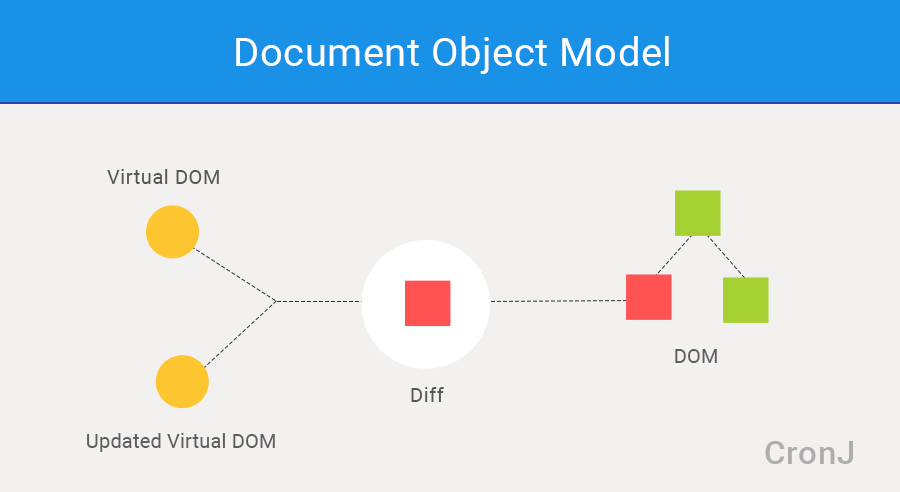
\includegraphics[width=14cm]{../Abbildungen/virtualDom.png}}
  \caption{React Virtual DOM}
  \label{React Virtual DOM}
\end{figure}
Resultat ist eine erheblich schnellere, effizientere und performantere DOM-Manipulation als frühere Lösungen. Das Virtual DOM kann fraglos als einer der Hauptgründe für Reacts Beliebtheit bezeichnet werden.
\subsection{Komponenten}

\subsection{Unidirektionaler Datenfluss}
Anders als viele der beliebten Frameworks verwendet React keinen bidirektionalen Datenfluss. Ebenso erstellt es in dem bekannten Model-View-Controller Konzept nur die View-Komponente und überlässt dem Entwickler die Wahl, ob und welche weiteren Komponenten verwendet werden. In einem bidirektionalen Datenfluss sind Model und View in direktem gegenseitigem Austausch, in dem Änderungen an einer Seite entsprechende Änderungen auf der anderen Seite auslösen. Diese gängige Lösung wird in den meisten Fällen gute Leistungen und Ergebnisse erzielen. Jedoch kann es hier zu unvorhersehbaren Datenflüssen kommen, eben weil sowohl Model als auch View Einfluss auf den Zustand der Anwendung haben. Es kann so zu nicht beabsichtigten Änderungen in nicht bearbeiteten Model-Bereichen und zu Kettenreaktionen von Updates kommen.\\
In React können Daten stattdessen nur in eine Richtung gegeben und verarbeitet werden, React ist also unidirektional. So wird ein Jonglieren der Zustände vermieden. \\
\begin{figure}[H]
     \centerline{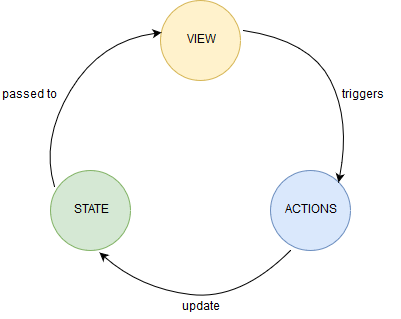
\includegraphics[width=12cm]{../Abbildungen/dataflow.png}}
  \caption{Unidirektionaler Datenfluss in React}
  \label{Unidirektionaler Datenfluss in React}
\end{figure}
\noindent Wie in Abbildung 2.2 zu sehen ist, fließen Daten hier in einem Kreislauf durch Zustand, View und Aktionen. Der Anwendungszustand, der die Zustände der Komponenten beinhaltet, wird an die View und ihre Child-Komponenten weitergegeben. In dieser werden Aktionen getriggered, beispielsweise durch den Nutzer, welche den Zustand verändern können. \\
Wie in 2.1 erwähnt konnte es vor React oftmals schwierig sein den Datenfluss in einer Anwendung nachzuverfolgen. Der unidirektionale Datenfluss Reacts schafft hier eine größere Nachvollziehbarkeit und begünstigt so Analyse und Fehlersuche. \\
\subsection{JSX}
JSX ist eine Syntax-Erweiterung zu JavaScript die für React empfehlenswert ist, da sie durch ihre Ähnlichkeit mit HTML-Syntax leicht zu lesen und verwenden ist. Der Typ eines Elements wird wie in HTML in einem öffnenden Tag festgelegt. Zwischen diesem öffnendem und dem abschließend folgenden schließendem Tag können die Kinder des Elements hinzugefügt werden. In Abbildung 2.3 ist als Beispiel eine ungeordnete Liste in JSX dargestellt.
\begin{figure}[!thb]
     \centerline{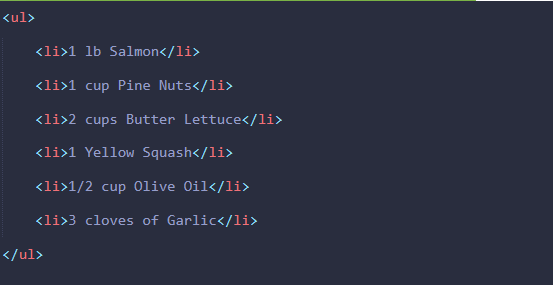
\includegraphics[width=12cm]{../Abbildungen/jsxList.png}}
  \caption{Ungeordnete Liste in JSX}
  \label{Ungeordnete Liste in JSX}
\end{figure}
In JSX werden JavaScript-Ausdrücke in geschweifte Klammern gestellt. Die Anzeige des Titel-Felds eines Elements wäre beispielsweise wie in Abbildung 2.4 umzusetzen.\\ 
\begin{figure}[!thb]
     \centerline{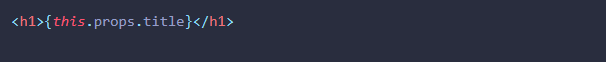
\includegraphics[width=12cm]{../Abbildungen/jsxExpression.png}}
  \caption{JavaScript in JSX}
  \label{JavaScript in JSX}
\end{figure}
Die Ausdrücke werden als vollwertiges Skript ausgeführt, es ist daher auch möglich vorher definierte Funktionen und vorimplementierte JavaScript Operationen an dieser Stelle zu verwenden. Da JSX eine Erweiterung zu JavaScript ist, kann in derartigen Funktionen auch JSX-Syntax verwendet werden. Wie in Abbildung 2.5 gezeigt, könnte beispielsweise eine Funktion setResult erstellt werden, die einen erhaltenen String untersucht und abhängig von dessen Inhalt zwei unterschiedliche JSX-Sequenzen ausgibt. \\
\section{React Native}
\section{Stärken}
\section{Kritik}
\section{Alternative Frameworks und Bibliotheken}
\section{Fazit}
